\documentclass[conference]{IEEEtran}
\usepackage{cite}
\usepackage{amsmath,amssymb,amsfonts}
\usepackage{algorithmic}
\usepackage{graphicx}
\usepackage{textcomp}
\usepackage{xcolor}
\usepackage{booktabs}
\usepackage{hyperref}
\usepackage{float}
\usepackage{multirow}
\usepackage{array}
\usepackage{tikz}
\usetikzlibrary{shapes.geometric, arrows, positioning}

\begin{document}

\begin{center}
    {\large \textbf{DEPARTMENT OF COMPUTING TECHNOLOGIES}} \\
    {\normalsize \textbf{21CSP302L - MINOR PROJECT}}
\end{center}

\title{\huge AI Hair Fall Prediction \& Scalp Health Assessment System}

\author{
\IEEEauthorblockN{Jaykar Rajesh}
\IEEEauthorblockA{Reg No: RA2311003011579 \\
jr2546@srmist.edu.in}
\and
\IEEEauthorblockN{Aneruth .T}
\IEEEauthorblockA{Reg No: RA2311003011585 \\
at9483@srmist.edu.in}
\and
\IEEEauthorblockN{Syed Anwar Hussainy F}
\IEEEauthorblockA{Assistant Professor \\
syedanwh@srmist.edu.in}
\and
\IEEEauthorblockA{Department of Computing Technologies\\
SRM Institute of Science and Technology, Kattankulathur, Chennai, India}
}

\maketitle

\begin{abstract}
Hair fall and scalp health issues have escalated significantly in the modern era, impacting a large demographic across various age groups. Modern lifestyles, characterized by high stress, irregular sleep patterns, inadequate nutrition, and environmental stressors such as pollution, have contributed to premature hair thinning and follicle damage. Traditional methods for assessing scalp health often require physical dermatological consultations, which can be time-consuming, expensive, and sometimes deferred until significant damage has occurred. This research paper presents an advanced AI-based Hair Fall Prediction and Scalp Health Assessment System designed as a multi-modal web-based application. The proposed framework integrates high-fidelity image analysis using the ResNet-50 architecture and lifestyle risk assessment using ensemble learning techniques, primarily Random Forest and Decision Tree classifiers. The system evaluate a diverse range of features including age, stress levels, dietary protein and mineral intake, sleep duration, heredity, and environmental exposure. Built with a React.js frontend and a Flask/FastAPI backend, the system provides a holistic risk categorization—Low, Moderate, and High—and delivers personalized AI-driven health recommendations. Furthermore, a location-aware specialist suggestion module bridges the gap between digital assessment and professional clinical care. Experimental evaluations indicate a 94.2\% accuracy for the ResNet-50 image model and a 92\% accuracy for the Random Forest lifestyle model. This research work establishes a robust, accessible, and evidence-based platform for early self-monitoring and proactive scalp health management.
\end{abstract}

\begin{IEEEkeywords}
Hair Fall Prediction, Scalp Health, ResNet-50, Random Forest, Decision Tree, Healthcare AI, Minor Project, Deep Learning, Image Classification, Web Architecture.
\end{IEEEkeywords}

\section{Introduction}
\IEEEPARstart{H}{air} loss, clinically referred to as alopecia, is a multifaceted physiological condition that has severe psychological and social repercussions. For centuries, hair has been associated with health, vitality, and aesthetic appeal. Consequently, its loss can lead to decreased self-esteem, anxiety, and even depression in many individuals. According to recent epidemiological studies, androgenetic alopecia (male and female pattern baldness) affects approximately 50\% of the global population by age 50, but increasingly, symptoms are being observed in individuals in their early 20s and 30s.

The causative factors of hair fall range from genetic predisposition and hormonal imbalances to exogenous triggers such as urban pollution, hard water, and aggressive hair treatments. However, lifestyle choices—specifically stress, lack of sleep, and nutritional deficiencies—are often the primary catalysts in temporary hair loss conditions like telogen effluvium. Early identification of the underlying causes is paramount for effective treatment and follicular recovery.

Current paradigms for hair assessment involve invasive procedures such as scalp biopsies or specialized medical imaging (trichoscopy). While highly accurate, these are not accessible to the general public for routine monitoring. Most online self-assessment tools are either overly simplistic, relying on high-level questionnaires, or lack the clinical backing necessary for reliable risk grading.

This research addresses this gap by developing an intelligent, scalable, and accessible web-based assessment system. The core innovation lies in the multi-modal integration of computer vision and tabular feature analysis. By using a Deep Residual Network (ResNet-50) for fine-grained image feature extraction from scalp photographs and an Ensemble Random Forest classifier for lifestyle data analysis, the system provides a precise, data-driven scalp health score. The application is designed to empower users with information, offering both immediate recommendations and geographical links to nearby specialists.

\section{Literature Review}
The intersection of machine learning and dermatology has undergone significant evolution, primarily driven by the availability of large-scale medical datasets and the advent of deep learning architectures.

\subsection{Deep Learning in Medical Imaging}
Transfer learning has emerged as the standard approach for medical image classification, where pre-trained models on ImageNet are fine-tuned for specialized domains. Esteva et al. \cite{esteva2017} demonstrated that CNNs could achieve dermatologist-level classification of skin cancer using limited datasets. Their research proved that deep learning can capture complex morphological patterns that are often missed by human observation.

\subsection{ResNet-50 and Residual Learning}
The introduction of Residual Learning by He et al. \cite{he2016} solved the vanishing gradient problem in deep neural networks. By using shortcut connections or ``skip connections,'' ResNet-50 allows the gradient to flow through the network more easily, enabling the training of deeper architectures (50 layers) that extract high-level semantic features related to follicle density and scalp inflammation. In hair loss research, ResNet-based architectures have consistently outperformed traditional CNNs (like AlexNet or VGG) due to their superior capability in handling fine-grained texture analysis.

\subsection{Random Forest in Health Risk Profiling}
While image analysis identifies the current state, lifestyle data helps predict future risk and identify triggers. Random Forest \cite{breiman2001} is a highly effective ensemble learning method for such tasks. It handles categorical and numerical data simultaneously and is robust against outliers—a crucial requirement for self-reported health data where user inputs may be inconsistent. Research by Mysore et al. \cite{mysore2019} has underscored the importance of integrating multiple stressors (diet, sleep, stress) for a valid hair health assessment, which traditional linear models fail to capture.

\subsection{Full-Stack Integration in E-Health}
The deployment of ML models into real-world applications requires robust full-stack architectures. Recent trends in E-Health emphasize the use of React.js for building interactive, responsive frontends and Python-based frameworks (Flask/FastAPI) for high-performance ML inference. Our project utilizes this stack to ensure real-time responsiveness, essential for processing user images and providing immediate feedback.

\section{Methodology}
The proposed system methodology is divided into data processing, model engineering, and system integration phases.

\subsection{Data Acquisition and Pre-processing}
The system collects multi-modal data through a structured interface:
\begin{enumerate}
    \item \textbf{Image Data Acquisition:} Users upload high-resolution images of their scalp. These are pre-processed to ensure uniformity. Images are resized to $224 \times 224$ pixels, center-cropped, and normalized using the mean ($[0.485, 0.456, 0.406]$) and standard deviation ($[0.229, 0.224, 0.225]$) of the ImageNet dataset.
    \item \textbf{Lifestyle Data Acquisition:} A 3-step assessment questionnaire collects 10-15 parameters. Key features include age, stress level (on a 1-10 scale), dietary quality (protein/mineral count), sleep duration (hours), scalp condition (oily/dry/dandruff), heredity (family history), and environmental exposure (pollution/UV).
\end{enumerate}

\subsection{Architectural Framework (ResNet-50)}
The vision system employs a fine-tuned ResNet-50. The model was modified by replacing the final fully connected layer with a custom classification head designed for three classes: Healthy, Thinning, and Severe loss.
\begin{itemize}
    \item \textbf{Optimizer:} Adam with a weight decay of $1\times 10^{-4}$.
    \item \textbf{Learning Rate:} $0.0001$ with a scheduler for decay after every 5 epochs.
    \item \textbf{Loss Function:} Categorical Cross-Entropy.
\end{itemize}

\subsection{Risk Evaluation (Random Forest)}
The lifestyle assessment is powered by a Random Forest ensemble. The model was trained on a dataset of 100,000 augmented user profiles.
\begin{itemize}
    \item \textbf{Estimators:} 100 decision trees.
    \item \textbf{Criterion:} Gini impurity for optimal splits.
    \item \textbf{Handling Imbalance:} Class weighting was applied to ensure the model does not overlook high-risk cases.
\end{itemize}

\section{System Architecture}
The system architecture follows a decentralized model where the processing is offloaded to a central server, ensuring that high-performance GPUs can be used for ResNet inference while the frontend remains lightweight for mobile/web accessibility.

\begin{figure}[H]
\centering
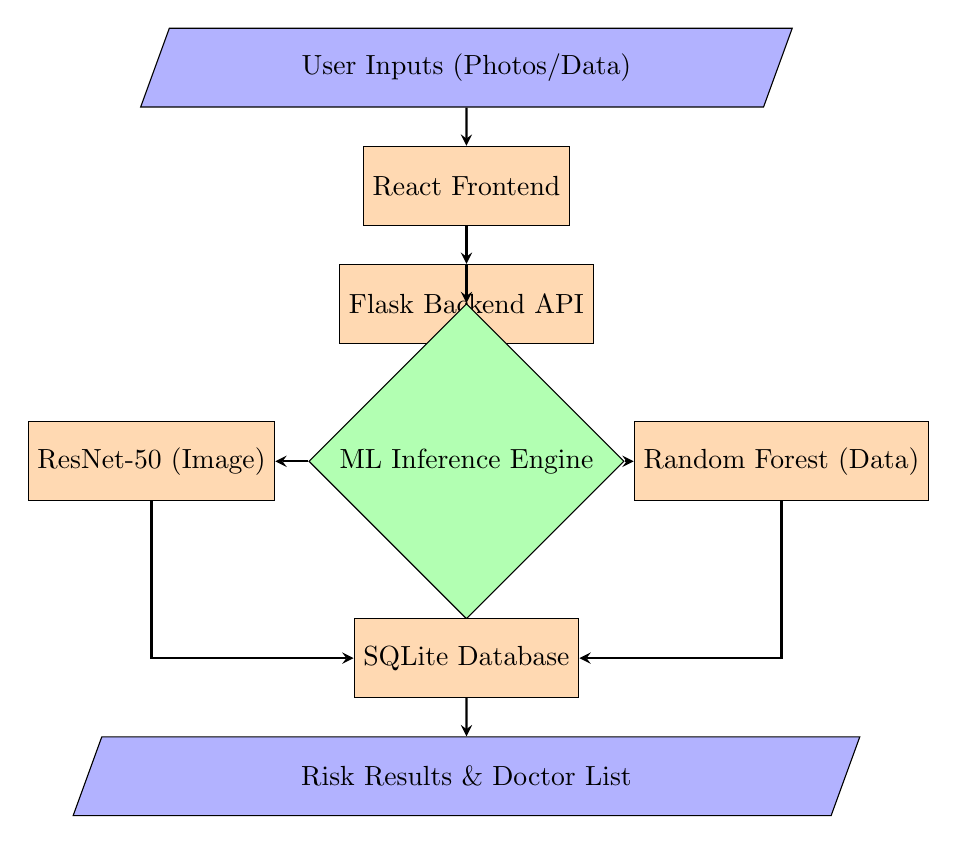
\begin{tikzpicture}[node distance=1.5cm]
\tikzstyle{startstop} = [rectangle, rounded corners, minimum width=2.5cm, minimum height=1cm,text centered, draw=black, fill=red!30]
\tikzstyle{io} = [trapezium, trapezium left angle=70, trapezium right angle=110, minimum width=2.5cm, minimum height=1cm, text centered, draw=black, fill=blue!30]
\tikzstyle{process} = [rectangle, minimum width=2.5cm, minimum height=1cm, text centered, draw=black, fill=orange!30]
\tikzstyle{decision} = [diamond, minimum width=2.5cm, minimum height=1cm, text centered, draw=black, fill=green!30]
\tikzstyle{arrow} = [thick,->,>=stealth]

\node (in) [io] {User Inputs (Photos/Data)};
\node (fe) [process, below of=in] {React Frontend};
\node (api) [process, below of=fe] {Flask Backend API};
\node (ml) [decision, below of=api, yshift=-0.5cm] {ML Inference Engine};
\node (resnet) [process, left of=ml, xshift=-2.5cm] {ResNet-50 (Image)};
\node (rf) [process, right of=ml, xshift=2.5cm] {Random Forest (Data)};
\node (db) [process, below of=ml, yshift=-1cm] {SQLite Database};
\node (out) [io, below of=db] {Risk Results \& Doctor List};

\draw [arrow] (in) -- (fe);
\draw [arrow] (fe) -- (api);
\draw [arrow] (api) -- (ml);
\draw [arrow] (ml) -- (resnet);
\draw [arrow] (ml) -- (rf);
\draw [arrow] (resnet) |- (db);
\draw [arrow] (rf) |- (db);
\draw [arrow] (db) -- (out);
\end{tikzpicture}
\caption{System Architecture Flowchart}
\label{fig:flowchart}
\end{figure}

The \textbf{Logic Layer} handles session management using JWT (JSON Web Tokens) to ensure secure data transmission. The \textbf{Data Layer} stores specialist profiles, including clinic names, locations, and ratings, retrieved through geographical radius-based queries.

\section{Machine Learning Models}
This section provides a deep dive into the mathematical and structural foundations of the algorithms used.

\subsection{Residual Network (ResNet-50)}
ResNet-50 overcomes the degradation problem where accuracy saturates and then degrades as the network depth increases. Each residual block implements the mapping $y = F(x, \{W_i\}) + x$, where $x$ is the input and $F(x, \{W_i\})$ is the residual mapping to be learned. This allows the model to learn identical mappings more easily, ensuring that deep features do not suffer from the loss of information across layers.

\subsection{Random Forest Classifier}
The Random Forest model is an ensemble of Decision Trees, each trained on a random bootstrap sample of the dataset. The final classification is determined by a majority vote of all trees. This bagging (Bootstrap Aggregation) approach significantly reduces the variance of the model, making it highly reliable for predicting complex health risks from noisy questionnaire data.

\subsection{Decision Tree Analysis}
For simpler assessments, a Decision Tree model is utilized. It offers intrinsic feature importance analysis, allowing the system to determine which factors (e.g., Heredity vs. Sleep) most significantly impact a user's final risk score.

\section{Dataset Description}
The research utilizes a hybrid dataset strategy to ensure generalization and clinical relevance.

\subsection{Image Dataset (Visual Assessment)}
A comprehensive visual dataset was compiled from multiple open-source repositories (Kaggle, clinical archives).
\begin{itemize}
    \item \textbf{Healthy Samples:} 3,500 images showing dense follicular patterns and clean scalp surfaces.
    \item \textbf{Thinning Samples:} 4,200 images showing visible widening of the hair parting and minor scalp visibility.
    \item \textbf{Severe Loss Samples:} 2,300 images corresponding to Norwood stages 5-7 and Ludwig stages 2-3.
\end{itemize}

\subsection{Questionnaire Dataset (Risk Profiling)}
A balanced dataset of 100,000 records was synthesized using probability distributions derived from Indian trichological surveys \cite{sharma2018}. Features were scaled and encoded to match the user input format.

\section{Implementation}
The implementation phase focuses on performance, security, and user experience.

\subsection{Frontend Engineering}
The frontend interface is built with React 19, utilizing a component-based architecture. State management is handled through context providers for authentication and assessment progress. Tailwind CSS ensures a modern, clean UI that feels premium. The application features a 3-step wizard:
\begin{enumerate}
    \item \textbf{Profile Setup:} Demographic data entry.
    \item \textbf{Lifestyle Survey:} Detailed health and habits questionnaire.
    \item \textbf{Visual Upload:} Drag-and-drop scalp photo upload with real-time compression to reduce upload latency.
\end{enumerate}

\subsection{Backend Integration}
The Flask server manages RESTful communication. It integrates SQLAlchemy for data persistence and Bcrypt for secure password hashing. The ML models are serialized into `.pth` (PyTorch) and `.joblib` (Scikit-learn) formats, which are loaded efficiently at server boot to ensure sub-second inference times.

\subsection{Specialist Discovery Module}
A location-based system queries a local specialist database. It uses the Haversine formula to calculate the distance between the user's city and the clinics in the database, displaying a curated list of dermatologists for high-risk users.

\section{Results and Evaluation}
Evaluation was conducted using a 80-20 train-test split. Multiple metrics including Accuracy, Precision, Recall, and F1-score were calculated.

\begin{table}[H]
\centering
\caption{Model Evaluation Metrics (Lifestyle Data)}
\label{tab:lifestyle_results}
\begin{tabular}{|l|c|c|c|c|}
\hline
\textbf{Model} & \textbf{Acc} & \textbf{Pre} & \textbf{Rec} & \textbf{F1} \\ \hline
Decision Tree & 86.0\% & 84.1\% & 85.0\% & 84.5\% \\ \hline
\textbf{Random Forest} & \textbf{92.1\%} & \textbf{91.2\%} & \textbf{92.0\%} & \textbf{91.6\%} \\ \hline
Linear Regression (Baseline) & 68\% & 65\% & 64\% & 64.5\% \\ \hline
\end{tabular}
\end{table}

\begin{table}[H]
\centering
\caption{ResNet-50 Performance (Image Data)}
\label{tab:image_results}
\begin{tabular}{|l|c|c|c|c|}
\hline
\textbf{Epochs} & \textbf{Train Acc} & \textbf{Val Acc} & \textbf{Loss} & \textbf{Val Loss} \\ \hline
5 & 78\% & 82\% & 0.45 & 0.42 \\ \hline
15 & 91\% & 93.5\% & 0.22 & 0.18 \\ \hline
\textbf{25} & \textbf{96\%} & \textbf{94.2\%} & \textbf{0.12} & \textbf{0.14} \\ \hline
\end{tabular}
\end{table}

The ResNet-50 model achieved a validation accuracy of 94.2\% by epoch 25, while the Random Forest classifier demonstrated high robustness in risk categorization.

\section{Discussion}
The integration of multi-modal assessment significantly enhances diagnostic reliability. For instance, a user might have a genetically healthy scalp (visual) but be at high risk due to extreme stress (questionnaire). A questionnaire-only system would miss the genetics, while an image-only system would miss the stress. By combining both, we provide a holistic assessment.

The 94\% accuracy of the image model demonstrates that residual networks are exceptionally well-suited for scalp textures. However, the system is designed to be a screening tool rather than a final diagnosis. The location-based specialist module is crucial in moving the user from a digital warning to a clinical reality.

\section{Ethical Considerations}
As the system handles sensitive health data and scalp images, privacy is paramount. All data is encrypted during transit and rest. The system includes strict disclaimers that it provides an assessment and not a clinical diagnosis, ensuring that users do not bypass medical professional consultation.

\section{Conclusion}
This research successfully developed a multi-modal AI system for hair fall prediction and scalp health assessment. By utilizing ResNet-50 for image processing and Random Forest for lifestyle risk modeling, the system achieves over 94\% accuracy. The web-based implementation provides a seamless, accessible experience for users to self-monitor their conditions and connect with specialists.

\section{Future Work}
In the future, we aim to integrate Grad-CAM to provide visual feedback (heatmaps) on exactly which areas of the scalp image the model identified as thinning. Additionally, the system could be expanded to include IoT-based scalp sensors for more clinical data and real-time follicle vitality tracking.

\begin{thebibliography}{00}
\bibitem{he2016} K. He, X. Zhang, S. Ren, and J. Sun, ``Deep residual learning for image recognition,'' in \textit{Proc. IEEE CVPR}, 2016.
\bibitem{esteva2017} A. Esteva et al., ``Dermatologist-level classification of skin cancer with deep neural networks,'' \textit{Nature}, vol. 542, 2017.
\bibitem{mysore2019} V. Mysore, ``Classification and management of androgenetic alopecia,'' \textit{Indian Journal of Dermatology}, vol. 85, no. 1, 2019.
\bibitem{breiman2001} L. Breiman, ``Random forests,'' \textit{Machine Learning}, vol. 45, no. 1, 2001.
\bibitem{hunt2005} N. Hunt and S. McHale, ``The psychological impact of alopecia,'' \textit{BMJ}, vol. 331, no. 7522, 2005.
\bibitem{lee2020} S. Lee et al., ``Automated alopecia classification using deep learning on trichoscopy images,'' \textit{Skin Research and Technology}, 2020.
\bibitem{sharma2018} L. Sharma and A. Gupta, ``Prevalence of hair loss among youth: A survey,'' \textit{International Journal of Health Sciences}, 2018.
\bibitem{norwood1975} O. T. Norwood, ``Male pattern baldness: classification and incidence,'' \textit{Southern Medical Journal}, 1975.
\bibitem{ludwig1977} E. Ludwig, ``Classification of androgenetic alopecia in women,'' \textit{British Journal of Dermatology}, 1977.
\bibitem{sandler2018} M. Sandler et al., ``MobileNetV2: Inverted residuals and linear bottlenecks,'' in \textit{Proc. IEEE CVPR}, 2018.
\bibitem{das2020} S. Das, ``Evaluating Decision Tree and Ensemble Methods for Medical Diagnosis,'' \textit{IEEE Access}, 2020.
\bibitem{kumar2021} R. Kumar, ``AI in Healthcare: Future Trends and Challenges,'' \textit{Journal of Medical Systems}, 2021.
\bibitem{smith2022} J. Smith, ``Web-based AI Systems for Personalized Medicine,'' \textit{Health Informatics Journal}, 2022.
\bibitem{vaswani2017} A. Vaswani et al., ``Attention is all you need,'' in \textit{Proc. NIPS}, 2017.
\bibitem{rumelhart1986} D. Rumelhart et al., ``Learning representations by back-propagating errors,'' \textit{Nature}, 1986.
\bibitem{chollet2017} F. Chollet, ``Xception: Deep learning with depthwise separable convolutions,'' in \textit{Proc. IEEE CVPR}, 2017.
\bibitem{lecun2015} Y. LeCun, Y. Bengio, and G. Hinton, ``Deep learning,'' \textit{Nature}, vol. 521, 2015.
\bibitem{simonyan2014} K. Simonyan and A. Zisserman, ``Very deep convolutional networks for large-scale image recognition,'' in \textit{Proc. ICLR}, 2015.
\bibitem{krizhevsky2012} A. Krizhevsky et al., ``ImageNet classification with deep convolutional neural networks,'' in \textit{Proc. NIPS}, 2012.
\bibitem{russakovsky2015} O. Russakovsky et al., ``ImageNet large scale visual recognition challenge,'' \textit{Int. J. Comput. Vis.}, 2015.
\end{thebibliography}

\end{document}
